\documentclass[svgnames,11pt]{beamer}
\input{/home/tof/Documents/Cozy/latex-include/preambule_commun.tex}
\input{/home/tof/Documents/Cozy/latex-include/preambule_beamer.tex}
%\usepackage{pgfpages} \setbeameroption{show notes on second screen=left}
\author[]{Christophe Viroulaud}
\title{Open Shortest First Path}
\date{\framebox{\textbf{Archi 13}}}
%\logo{}
\institute{Terminale - NSI}

\begin{document}
\begin{frame}
    \titlepage
\end{frame}

\begin{frame}
    \frametitle{Le protocole RIP souffre de plusieurs limitations}

    \begin{framed}
        \centering Quelle solution mettre en place pour surmonter ces limitations?
    \end{framed}

\end{frame}

\section{Bande passante}

\begin{frame}
    \frametitle{Bande passante}

    \begin{aretenir}[]
        La \emph{bande passante} est la quantité d'information qui peut être transmise par unité de temps. Elle se mesure en \emph{bits par seconde (bit/s)}.
    \end{aretenir}

\end{frame}

\begin{frame}
    On définira maintenant le \emph{coût d'une liaison} pour relier deux routeurs.

    \begin{aretenir}[]
        Le coût d'une liaison est calculé par la relation :
        $$\dfrac{10^8}{\mbox{bande passante}}$$
        Dans le cas d'une connexion asymétrique on utilise le débit descendant.
    \end{aretenir}
    \note{La valeur $10^8$ a été choisie pour donner un coût de 1 à une liaison FastEthernet de 100Mbit/s.}
\end{frame}


\begin{frame}
    \frametitle{}

    \begin{activite}
        Calculer les coûts des connexions suivantes :
        \begin{itemize}
            \item satellite 50Mbit/s,
            \item câble Éthernet 10Mbit/s,
            \item modem 62500bit/s,
            \item fibre optique 1Gbit/s,
            \item ADSL 13Mbit/s (descendant), 1Mbit/s (montant).
        \end{itemize}
    \end{activite}

\end{frame}

\begin{frame}
    \frametitle{Correction}

    \begin{itemize}
        \item satellite 50Mbit/s: $\dfrac{10^8}{5×10^7}=2$,
        \item câble Éthernet 10Mbit/s: $\dfrac{10^8}{10^7}=10$,
        \item modem 62500bit/s: $\dfrac{10^8}{6,25×10^4}=1600$,
        \item fibre optique 1Gbit/s: $\dfrac{10^8}{10^9}=0,1$,
        \item ADSL 13Mbit/s (descendant), 1Mbit/s (montant): $\dfrac{10^8}{1,3×10^7}=7,7$.
    \end{itemize}
    \note[item]{câble éthernet:10Mbit/s, 100Mbit/s, 1Gbit/s}
    \note[item]{jusqu'à 10Gbit/s}
\end{frame}
\section{Open Shortest Path First}
\subsection{Principe}
\begin{frame}
    \frametitle{Open Shortest Path First - Principe}

    \begin{itemize}
        \item<1-> Le protocole OSPF a été développé dans les années 90 pour pallier les difficultés du protocole RIP.
        \item<2-> C'est un \textbf{routage à état de lien:}\begin{itemize}
            \item mise à jour seulement quand il y a une modification,
            \item table de routage en fonction du coût de liaison. 
        \end{itemize}
    \end{itemize}

    \note{rappel: RIP : routage à vecteur de distance}
\end{frame}
\subsection{Organisation en zones}
\begin{frame}
    \frametitle{Organisation en zones}

    \begin{center}
        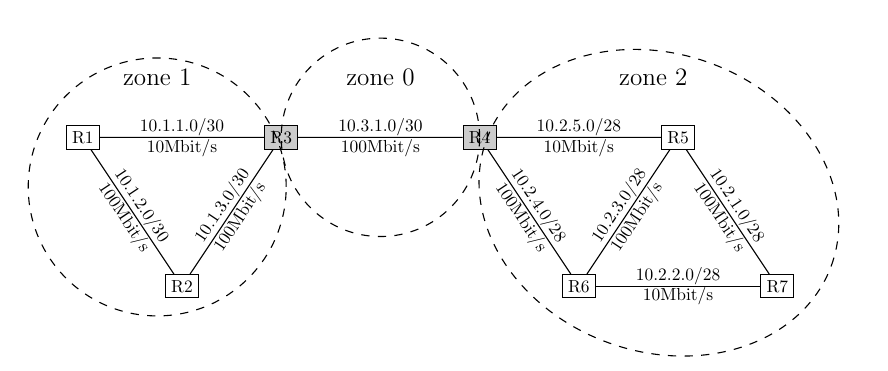
\begin{tikzpicture}[scale=0.63, transform shape]
            \node[draw] (R1) at (-6,3) {R1};
            \node[draw] (R2) at (-4,0) {R2};
            \node[draw, fill=gray!40] (R3) at (-2,3) {R3};
            \node[draw, fill=gray!40] (R4) at (2,3) {R4};
            \node[draw] (R5) at (6,3) {R5};
            \node[draw] (R6) at (4,0) {R6};
            \node[draw] (R7) at (8,0) {R7};
            \node (Z1) at (-4.5,4.2) {\Large{zone 1}};
            \node (Z0) at (0,4.2) {\Large{zone 0}};
            \node (Z2) at (5.5,4.2) {\Large{zone 2}};

            \draw (R1) -- (R3) node[midway,text width=1.8cm, text centered]{10.1.1.0/30 10Mbit/s};
            \draw (R1) -- (R2) node[sloped, midway,text width=1.8cm, text centered]{10.1.2.0/30 100Mbit/s};
            \draw (R3) -- (R2) node[sloped, midway,text width=1.8cm, text centered]{10.1.3.0/30 100Mbit/s};
            \draw (R3) -- (R4) node[midway,text width=1.8cm, text centered]{10.3.1.0/30 100Mbit/s};
            \draw (R4) -- (R5) node[midway,text width=1.8cm, text centered]{10.2.5.0/28 10Mbit/s};
            \draw (R4) -- (R6) node[sloped, midway,text width=1.8cm, text centered]{10.2.4.0/28 100Mbit/s};
            \draw (R5) -- (R6) node[sloped, midway,text width=1.8cm, text centered]{10.2.3.0/28 100Mbit/s};
            \draw (R7) -- (R6) node[midway,text width=1.8cm, text centered]{10.2.2.0/28 10Mbit/s};
            \draw (R5) -- (R7) node[sloped, midway,text width=1.8cm, text centered]{10.2.1.0/28 100Mbit/s};

            \draw[dashed] (0,3) circle (2) ;
            \draw[dashed] (-4.5,2) circle (2.6) ;
            \draw[dashed,rotate=-20] (4.7,3.5) ellipse (3.7 and 3) ;
        \end{tikzpicture}
        \captionof{figure}{Découpage en zones}
        \label{zone}
    \end{center}
    
\end{frame}
\begin{frame}
    \frametitle{}

    \begin{aretenir}[]
        Chaque zone a un numéro unique. La zone 0, appelée \textbf{Backbone}, est la zone centrale à laquelle toutes les autres zones sont connectées à l'aide d’un routeur particulier appelé \textbf{ABR (Area Border Router)}.
    \end{aretenir}

\end{frame}

\subsection{Découverte du réseau}
\subsubsection{Identificateur}
\begin{frame}
    \frametitle{Identificateur}

    \begin{aretenir}[]
        Chaque routeur est repéré par un identificateur unique (R1\dots). 
    \end{aretenir}
    \begin{aretenir}[Remarque]
    En pratique l'identificateur est la plus grande adresse IP parmi celles des interfaces réseaux du routeur.
    \end{aretenir}
\note{Attention c'est bien une étiquette et pas une adresse en tant que tel. ex: pour R2: 10.1.2.2}
\end{frame}

\subsubsection{Message HELLO}
\begin{frame}
    \frametitle{Message HELLO}
    \begin{aretenir}[]
        Chaque routeur envoie des paquets de type \textbf{HELLO} à travers toutes ses interfaces. À
        réception de la réponse il établit une relation de voisinage.
    \end{aretenir}
    \begin{center}
        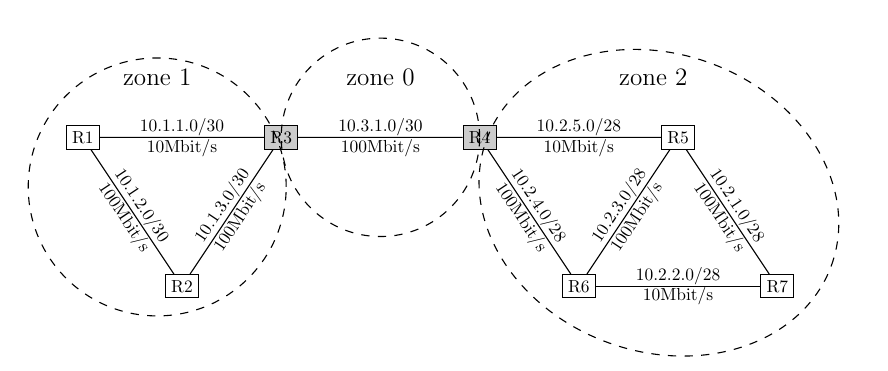
\begin{tikzpicture}[scale=0.63, transform shape]
            \node[draw] (R1) at (-6,3) {R1};
            \node[draw] (R2) at (-4,0) {R2};
            \node[draw, fill=gray!40] (R3) at (-2,3) {R3};
            \node[draw, fill=gray!40] (R4) at (2,3) {R4};
            \node[draw] (R5) at (6,3) {R5};
            \node[draw] (R6) at (4,0) {R6};
            \node[draw] (R7) at (8,0) {R7};
            \node (Z1) at (-4.5,4.2) {\Large{zone 1}};
            \node (Z0) at (0,4.2) {\Large{zone 0}};
            \node (Z2) at (5.5,4.2) {\Large{zone 2}};

            \draw (R1) -- (R3) node[midway,text width=1.8cm, text centered]{10.1.1.0/30 10Mbit/s};
            \draw (R1) -- (R2) node[sloped, midway,text width=1.8cm, text centered]{10.1.2.0/30 100Mbit/s};
            \draw (R3) -- (R2) node[sloped, midway,text width=1.8cm, text centered]{10.1.3.0/30 100Mbit/s};
            \draw (R3) -- (R4) node[midway,text width=1.8cm, text centered]{10.3.1.0/30 100Mbit/s};
            \draw (R4) -- (R5) node[midway,text width=1.8cm, text centered]{10.2.5.0/28 10Mbit/s};
            \draw (R4) -- (R6) node[sloped, midway,text width=1.8cm, text centered]{10.2.4.0/28 100Mbit/s};
            \draw (R5) -- (R6) node[sloped, midway,text width=1.8cm, text centered]{10.2.3.0/28 100Mbit/s};
            \draw (R7) -- (R6) node[midway,text width=1.8cm, text centered]{10.2.2.0/28 10Mbit/s};
            \draw (R5) -- (R7) node[sloped, midway,text width=1.8cm, text centered]{10.2.1.0/28 100Mbit/s};

            \draw[dashed] (0,3) circle (2) ;
            \draw[dashed] (-4.5,2) circle (2.6) ;
            \draw[dashed,rotate=-20] (4.7,3.5) ellipse (3.7 and 3) ;
        \end{tikzpicture}
    \end{center}
    
    \note[item]{découverte voisinage immédiat = initialisation}
    \note[item]{un message HELLO toutes les 10s}
\end{frame}
\begin{frame}
    \frametitle{}

    \begin{center}
        \begin{tabular}{|*{4}{c|}}
            \hline
            Lien    & Sous-réseau & Coût & Zone \\
            \hline
            R1 - R2 & 10.1.2.0/30 & 1    & 1    \\
            \hline
            R1 - R3 & 10.1.1.0/30 & 10   & 1    \\
            \hline
        \end{tabular}
        \captionof{table}{Relations de voisinage immédiates pour R1}
    \end{center}    

\end{frame}
\begin{frame}
    \frametitle{}

    \begin{aretenir}[Remarque]
        C'est également lors de cette étape que les routeurs \emph{ABR} annoncent leur rôle aux autres.
    \end{aretenir}

\end{frame}
\begin{frame}
    \frametitle{HELLO}

    \begin{activite}
        Établir le tableau des relations de voisinage pour R5.
    \end{activite}


\end{frame}

\begin{frame}
    \frametitle{Correction}

    \begin{center}
        \begin{tabular}{|*{4}{c|}}
            \hline
            Lien    & Sous-réseau & Coût & Zone \\
            \hline
            R5 - R4 & 10.2.5.0/28 & 10   & 2    \\
            \hline
            R5 - R6 & 10.2.3.0/28 & 1    & 2    \\
            \hline
            R5 - R7 & 10.2.1.0/28 & 1    & 2    \\
            \hline
        \end{tabular}
        \captionof{table}{Relations de voisinage pour R5}
    \end{center}

\end{frame}

\begin{frame}
    \frametitle{Réponse à HELLO}

    Quand un routeur de la zone reçoit un paquet HELLO:
    \begin{center}
        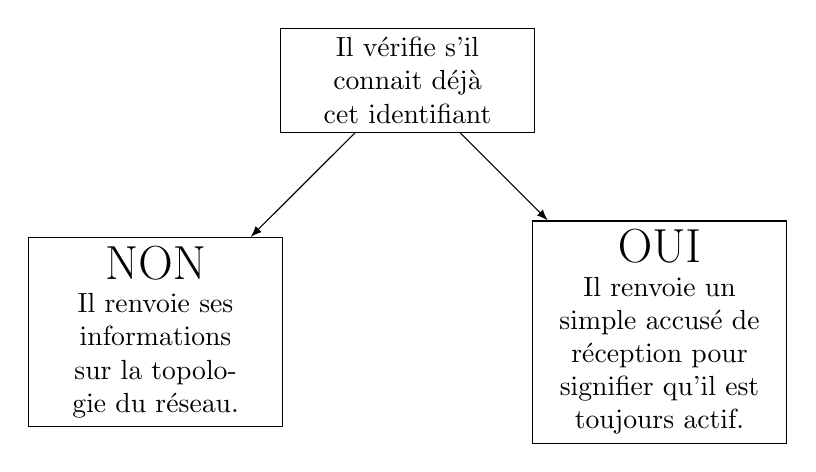
\begin{tikzpicture}[scale=0.8]
            \node[draw, text width=3cm, text centered] (1) at (0,0) {Il vérifie s'il connait déjà cet identifiant};
            \node[draw, text width=3cm, text centered] (2) at (-4,-4) {{\LARGE NON}\\ Il renvoie ses informations sur la topologie du réseau.};
            \node[draw, text width=3cm, text centered] (3) at (4,-4) {{\LARGE OUI}\\ Il renvoie un simple accusé de réception pour signifier qu'il est toujours actif.};

            \draw[->,>=latex] (1) -- (2);
            \draw[->,>=latex] (1) -- (3);
        \end{tikzpicture}
    \end{center}

\end{frame}
\subsubsection{LSA}
\begin{frame}
    \frametitle{LSA: État de lien de communication}
    \begin{aretenir}[]
        Les messages qui contiennent les \emph{informations sur la topologie du réseau} sont appelés \textbf{LSA (Link State Advertisement)}.
        Ces échanges sont \emph{limités à la zone à laquelle appartient le routeur}.
    \end{aretenir}

\end{frame}
\begin{frame}
    \frametitle{}
    \begin{center}
        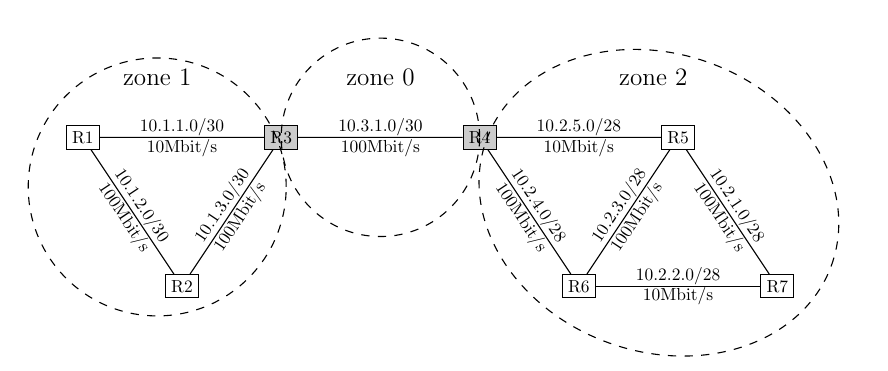
\begin{tikzpicture}[scale=0.63, transform shape]
            \node[draw] (R1) at (-6,3) {R1};
            \node[draw] (R2) at (-4,0) {R2};
            \node[draw, fill=gray!40] (R3) at (-2,3) {R3};
            \node[draw, fill=gray!40] (R4) at (2,3) {R4};
            \node[draw] (R5) at (6,3) {R5};
            \node[draw] (R6) at (4,0) {R6};
            \node[draw] (R7) at (8,0) {R7};
            \node (Z1) at (-4.5,4.2) {\Large{zone 1}};
            \node (Z0) at (0,4.2) {\Large{zone 0}};
            \node (Z2) at (5.5,4.2) {\Large{zone 2}};

            \draw (R1) -- (R3) node[midway,text width=1.8cm, text centered]{10.1.1.0/30 10Mbit/s};
            \draw (R1) -- (R2) node[sloped, midway,text width=1.8cm, text centered]{10.1.2.0/30 100Mbit/s};
            \draw (R3) -- (R2) node[sloped, midway,text width=1.8cm, text centered]{10.1.3.0/30 100Mbit/s};
            \draw (R3) -- (R4) node[midway,text width=1.8cm, text centered]{10.3.1.0/30 100Mbit/s};
            \draw (R4) -- (R5) node[midway,text width=1.8cm, text centered]{10.2.5.0/28 10Mbit/s};
            \draw (R4) -- (R6) node[sloped, midway,text width=1.8cm, text centered]{10.2.4.0/28 100Mbit/s};
            \draw (R5) -- (R6) node[sloped, midway,text width=1.8cm, text centered]{10.2.3.0/28 100Mbit/s};
            \draw (R7) -- (R6) node[midway,text width=1.8cm, text centered]{10.2.2.0/28 10Mbit/s};
            \draw (R5) -- (R7) node[sloped, midway,text width=1.8cm, text centered]{10.2.1.0/28 100Mbit/s};

            \draw[dashed] (0,3) circle (2) ;
            \draw[dashed] (-4.5,2) circle (2.6) ;
            \draw[dashed,rotate=-20] (4.7,3.5) ellipse (3.7 and 3) ;
        \end{tikzpicture}
    \end{center}
    

\end{frame}
\begin{frame}
    \frametitle{}
Le routeur R1 reçoit les messages LSA de R2 et R3.
    \begin{center}
        \begin{tabular}{|*{4}{c|}}
            \hline
            Lien    & Sous-réseau & Coût & Zone \\
            \hline
            R1 - R2 & 10.1.2.0/30 & 1    & 1    \\
            \hline
            R1 - R3 & 10.1.1.0/30 & 10   & 1    \\
            \hline
            R2 - R3 & 10.1.3.0/30 & 1    & 1    \\
            \hline
        \end{tabular}
        \captionof{table}{Topologie pour R1}
    \end{center}
    \begin{aretenir}[]
        Il faut plusieurs échanges HELLO (donc plusieurs messages LSA) pour obtenir une vision globale \textbf{de la zone}.
    \end{aretenir}
\end{frame}

\begin{frame}
    \frametitle{}

    \begin{activite}
        Établir la vision de la topologie du réseau pour R5.
    \end{activite}

\end{frame}

\begin{frame}
    \frametitle{Correction}

    \begin{center}
        \begin{tabular}{|*{4}{c|}}
            \hline
            Lien    & Sous-réseau & Coût & Zone \\
            \hline
            R5 - R4 & 10.2.5.0/28 & 10   & 2    \\
            \hline
            R5 - R6 & 10.2.3.0/28 & 1    & 2    \\
            \hline
            R5 - R7 & 10.2.1.0/28 & 1    & 2    \\
            \hline
            R4 - R6 & 10.2.4.0/28 & 1    & 2    \\
            \hline
            R6 - R7 & 10.2.2.0/28 & 10    & 2    \\
            \hline
        \end{tabular}
        \captionof{table}{Topologie pour R5}
    \end{center}

\end{frame}

\subsection{Calculs des meilleurs routes}

\begin{frame}
    \frametitle{}

    \begin{aretenir}[]
        Chaque routeur calcule ensuite la meilleure route pour atteindre chaque réseau. 
        \textbf{L'algorithme de Dijkstra} -établi en 1959- permet de trouver le plus court chemin entre deux sommets d'un graphe pondéré.
    \end{aretenir}
\note{Nous verrons le fonctionnement plus tard.}
\end{frame}

\begin{frame}
    \frametitle{Dans la zone}
    \begin{center}
        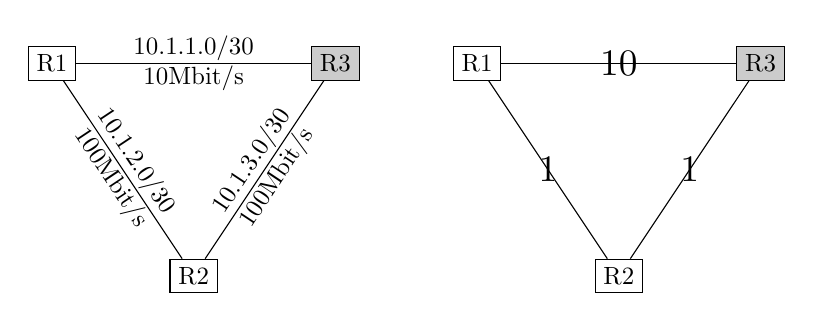
\begin{tikzpicture}[scale=0.9, transform shape]
            \node[draw] (R1) at (-6,3) {R1};
            \node[draw] (R2) at (-4,0) {R2};
            \node[draw, fill=gray!40] (R3) at (-2,3) {R3};

            \draw (R1) -- (R3) node[midway, scale=1.5]{10};
            \draw (R1) -- (R2) node[midway, scale=1.5]{1};
            \draw (R3) -- (R2) node[midway, scale=1.5]{1};


            \node[draw] (R1b) at (-12,3) {R1};
            \node[draw] (R2b) at (-10,0) {R2};
            \node[draw, fill=gray!40] (R3b) at (-8,3) {R3};
            \draw (R1b) -- (R3b) node[midway,text width=1.8cm, text centered]{10.1.1.0/30 10Mbit/s};
            \draw (R1b) -- (R2b) node[sloped, midway,text width=1.8cm, text centered]{10.1.2.0/30 100Mbit/s};
            \draw (R3b) -- (R2b) node[sloped, midway,text width=1.8cm, text centered]{10.1.3.0/30 100Mbit/s};
        \end{tikzpicture}
        \captionof{figure}{Graphe pondéré de la zone 1}
        \label{zone1}
    \end{center}
    \note{coûts des chemins}
\end{frame}

\begin{frame}
    \frametitle{Dans la zone}
    \begin{center}
        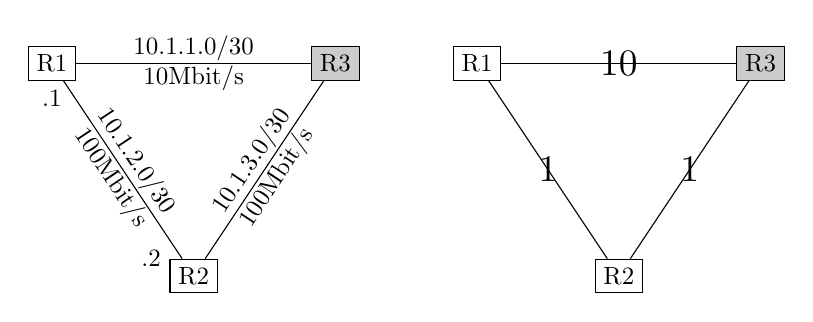
\begin{tikzpicture}[scale=0.9, transform shape]
            \node[draw] (R1) at (-6,3) {R1};
            \node[draw] (R2) at (-4,0) {R2};
            \node[draw, fill=gray!40] (R3) at (-2,3) {R3};

            \draw (R1) -- (R3) node[midway, scale=1.5]{10};
            \draw (R1) -- (R2) node[midway, scale=1.5]{1};
            \draw (R3) -- (R2) node[midway, scale=1.5]{1};
            \node (R1adr) at (-12,2.5) {.1};
            \node (R2adr) at (-10.6,0.25) {.2};

            \node[draw] (R1b) at (-12,3) {R1};
            \node[draw] (R2b) at (-10,0) {R2};
            \node[draw, fill=gray!40] (R3b) at (-8,3) {R3};
            \draw (R1b) -- (R3b) node[midway,text width=1.8cm, text centered]{10.1.1.0/30 10Mbit/s};
            \draw (R1b) -- (R2b) node[sloped, midway,text width=1.8cm, text centered]{10.1.2.0/30 100Mbit/s};
            \draw (R3b) -- (R2b) node[sloped, midway,text width=1.8cm, text centered]{10.1.3.0/30 100Mbit/s};
        \end{tikzpicture}
        \captionof{figure}{Graphe pondéré de la zone 1}
        \label{zone1}
    \end{center}
    Le routeur R1 calcule le chemin le plus court pour atteindre chaque réseau de la zone 1.
    \begin{center}
        \begin{tabular}{|*{4}{c|}}
            \hline
            Destination & Passerelle    & Interface & Coût \\
            \hline
            10.1.2.0/30 &               & 10.1.2.1  & 1    \\
            \hline
            10.1.3.0/30 & R2 & 10.1.2.1  & 2    \\
            \hline
            10.1.1.0/30 &               & 10.1.1.1  & 10   \\
            \hline
        \end{tabular}
        \captionof{table}{Table de routage de R1}
    \end{center}

    \note[item]{Les adresses 10.1.2.1 et 10.1.2.2 correspondent aux interfaces (de respectivement R1 et R2) sur le réseau 10.1.2.0/30 (vue quand on a donné des identifiants).\\
        L'adresse 10.1.1.1 correspond à l'interface de R1 sur le réseau 10.1.1.0/30.}
    \note[item]{Dans la littérature, les écritures peuvent varier: ainsi la destination peut être un routeur et non un réseau (voir sujet zéro 2021) $\rightarrow$ exemples dans les exercices Nous gardons ici la même écriture que pour RIP.}
\end{frame}


\begin{frame}
    \frametitle{}
    \begin{activite}
        Établir la table de routage de R5 dans sa zone.
    \end{activite}
\begin{center}
    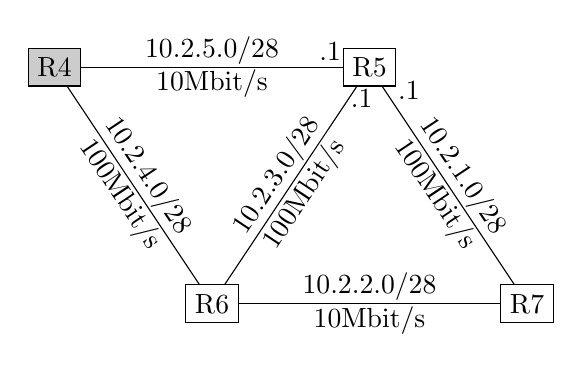
\begin{tikzpicture}
        \node[draw, fill=gray!40] (R4) at (2,3) {R4};
        \node[draw] (R5) at (6,3) {R5};
        \node[draw] (R6) at (4,0) {R6};
        \node[draw] (R7) at (8,0) {R7};
        \node (int1) at (5.5,3.2) {.1};
        \node (int2) at (5.9,2.6) {.1};
        \node (int3) at (6.5,2.7) {.1};

        \draw (R4) -- (R5) node[midway,text width=1.8cm, text centered]{10.2.5.0/28 10Mbit/s};
        \draw (R4) -- (R6) node[sloped, midway,text width=1.8cm, text centered]{10.2.4.0/28 100Mbit/s};
        \draw (R5) -- (R6) node[sloped, midway,text width=1.8cm, text centered]{10.2.3.0/28 100Mbit/s};
        \draw (R7) -- (R6) node[midway,text width=1.8cm, text centered]{10.2.2.0/28 10Mbit/s};
        \draw (R5) -- (R7) node[sloped, midway,text width=1.8cm, text centered]{10.2.1.0/28 100Mbit/s};
    \end{tikzpicture}
\end{center}

\end{frame}

\begin{frame}
    \frametitle{Correction}
Première étape: dans la zone
    \begin{center}
        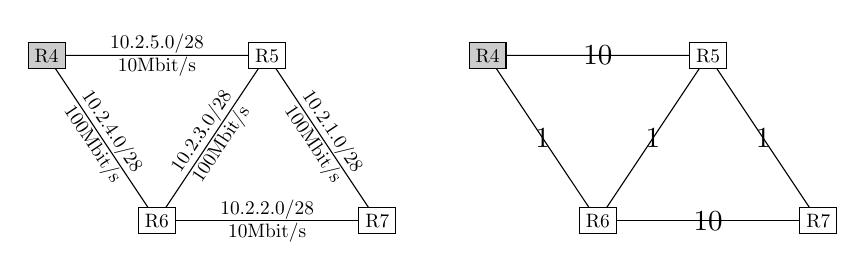
\begin{tikzpicture}[scale=0.7, transform shape]
            \node[draw, fill=gray!40] (R4) at (2,3) {R4};
            \node[draw] (R5) at (6,3) {R5};
            \node[draw] (R6) at (4,0) {R6};
            \node[draw] (R7) at (8,0) {R7};

            \draw (R4) -- (R5) node[midway,text width=1.8cm, text centered]{10.2.5.0/28 10Mbit/s};
            \draw (R4) -- (R6) node[sloped, midway,text width=1.8cm, text centered]{10.2.4.0/28 100Mbit/s};
            \draw (R5) -- (R6) node[sloped, midway,text width=1.8cm, text centered]{10.2.3.0/28 100Mbit/s};
            \draw (R7) -- (R6) node[midway,text width=1.8cm, text centered]{10.2.2.0/28 10Mbit/s};
            \draw (R5) -- (R7) node[sloped, midway,text width=1.8cm, text centered]{10.2.1.0/28 100Mbit/s};

            \node[draw, fill=gray!40] (R4b) at (10,3) {R4};
            \node[draw] (R5b) at (14,3) {R5};
            \node[draw] (R6b) at (12,0) {R6};
            \node[draw] (R7b) at (16,0) {R7};

            \draw (R4b) -- (R5b) node[midway, scale=1.5]{10};
            \draw (R4b) -- (R6b) node[midway, scale=1.5]{1};
            \draw (R5b) -- (R6b) node[midway, scale=1.5]{1};
            \draw (R7b) -- (R6b) node[midway, scale=1.5]{10};
            \draw (R5b) -- (R7b) node[midway, scale=1.5]{1};
        \end{tikzpicture}
        \captionof{figure}{Graphe pondéré de la zone 2}
        \label{zone2}
    \end{center}

    \begin{center}
        \begin{tabular}{|*{4}{c|}}
            \hline
            Destination & Passerelle    & Interface & Coût \\
            \hline
            10.2.1.0/28 &               & 10.2.1.1  & 1    \\
            \hline
            10.2.2.0/28 & R7 & 10.2.1.1  & 11    \\
            \hline
            10.2.3.0/28 &               & 10.2.3.1  & 1   \\
            \hline
            10.2.4.0/28 & R6 & 10.2.3.1  & 2    \\
            \hline
            10.2.5.0/28 &  & 10.2.5.1  & 10    \\
            \hline
        \end{tabular}
        \captionof{table}{Table de routage de R5}
    \end{center}
    \note[item]{Pour atteindre 10.2.2.0, on pouvait également passer par R6.}
    \note[item]{Les interfaces 100Mbit/s $\rightarrow$ FastEthernet}
\end{frame}

\begin{frame}
    \frametitle{Depuis les autres zones}
\begin{center}
    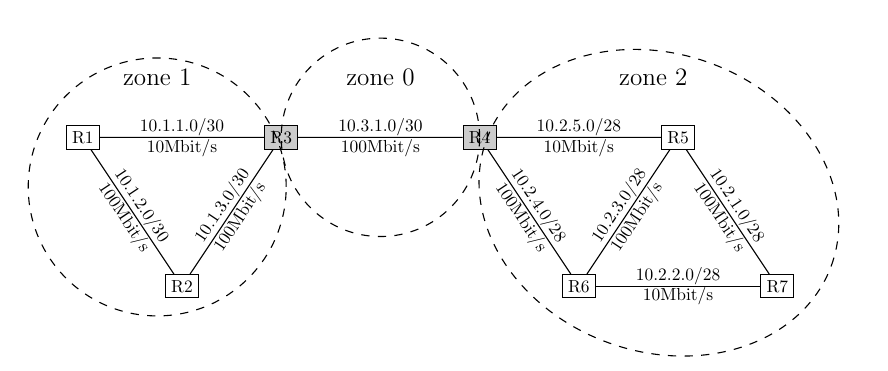
\begin{tikzpicture}[scale=0.63, transform shape]
        \node[draw] (R1) at (-6,3) {R1};
        \node[draw] (R2) at (-4,0) {R2};
        \node[draw, fill=gray!40] (R3) at (-2,3) {R3};
        \node[draw, fill=gray!40] (R4) at (2,3) {R4};
        \node[draw] (R5) at (6,3) {R5};
        \node[draw] (R6) at (4,0) {R6};
        \node[draw] (R7) at (8,0) {R7};
        \node (Z1) at (-4.5,4.2) {\Large{zone 1}};
        \node (Z0) at (0,4.2) {\Large{zone 0}};
        \node (Z2) at (5.5,4.2) {\Large{zone 2}};

        \draw (R1) -- (R3) node[midway,text width=1.8cm, text centered]{10.1.1.0/30 10Mbit/s};
        \draw (R1) -- (R2) node[sloped, midway,text width=1.8cm, text centered]{10.1.2.0/30 100Mbit/s};
        \draw (R3) -- (R2) node[sloped, midway,text width=1.8cm, text centered]{10.1.3.0/30 100Mbit/s};
        \draw (R3) -- (R4) node[midway,text width=1.8cm, text centered]{10.3.1.0/30 100Mbit/s};
        \draw (R4) -- (R5) node[midway,text width=1.8cm, text centered]{10.2.5.0/28 10Mbit/s};
        \draw (R4) -- (R6) node[sloped, midway,text width=1.8cm, text centered]{10.2.4.0/28 100Mbit/s};
        \draw (R5) -- (R6) node[sloped, midway,text width=1.8cm, text centered]{10.2.3.0/28 100Mbit/s};
        \draw (R7) -- (R6) node[midway,text width=1.8cm, text centered]{10.2.2.0/28 10Mbit/s};
        \draw (R5) -- (R7) node[sloped, midway,text width=1.8cm, text centered]{10.2.1.0/28 100Mbit/s};

        \draw[dashed] (0,3) circle (2) ;
        \draw[dashed] (-4.5,2) circle (2.6) ;
        \draw[dashed,rotate=-20] (4.7,3.5) ellipse (3.7 and 3) ;
    \end{tikzpicture}
    
        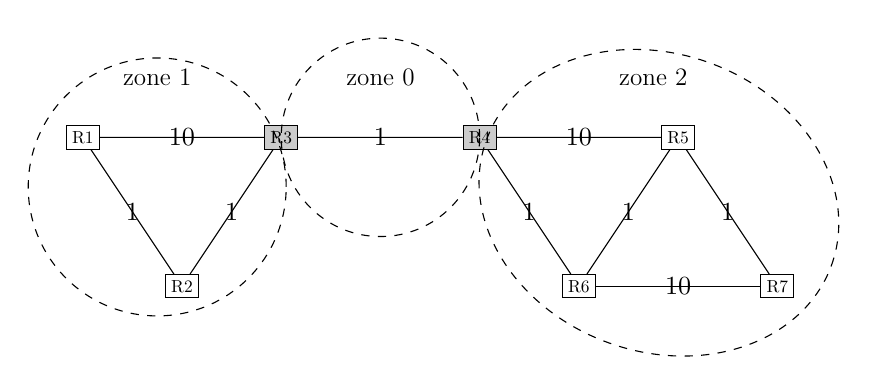
\begin{tikzpicture}[scale=0.63, transform shape]
            \node[draw] (R1) at (-6,3) {R1};
            \node[draw] (R2) at (-4,0) {R2};
            \node[draw, fill=gray!40] (R3) at (-2,3) {R3};
            \node[draw, fill=gray!40] (R4) at (2,3) {R4};
            \node[draw] (R5) at (6,3) {R5};
            \node[draw] (R6) at (4,0) {R6};
            \node[draw] (R7) at (8,0) {R7};
            \node (Z1) at (-4.5,4.2) {\Large{zone 1}};
            \node (Z0) at (0,4.2) {\Large{zone 0}};
            \node (Z2) at (5.5,4.2) {\Large{zone 2}};

            \draw (R1) -- (R3) node[midway,scale=1.5]{10};
            \draw (R1) -- (R2) node[midway,scale=1.5]{1};
            \draw (R3) -- (R2) node[midway,scale=1.5]{1};
            \draw (R3) -- (R4) node[midway,scale=1.5]{1};
            \draw (R4) -- (R5) node[midway,scale=1.5]{10};
            \draw (R4) -- (R6) node[midway,scale=1.5]{1};
            \draw (R5) -- (R6) node[midway,scale=1.5]{1};
            \draw (R7) -- (R6) node[midway,scale=1.5]{10};
            \draw (R5) -- (R7) node[midway,scale=1.5]{1};

            \draw[dashed] (0,3) circle (2) ;
            \draw[dashed] (-4.5,2) circle (2.6) ;
            \draw[dashed,rotate=-20] (4.7,3.5) ellipse (3.7 and 3) ;
        \end{tikzpicture}
    \end{center}

\end{frame}
\begin{frame}
    \frametitle{Depuis les autres zones}
    Le routeur \emph{de bordure} R3 communique les plus courts chemins (passant par lui) vers la zone 2. Le routeur R1 complète alors sa table de routage.
    \begin{center}
        \begin{tabular}{|*{4}{c|}}
            \hline
            Destination & Passerelle    & Interface & Coût \\
            \hline
            10.1.2.0/30 &               & 10.1.2.1  & 1    \\
            \hline
            10.1.3.0/30 & R2 & 10.1.2.1  & 2    \\
            \hline
            10.1.1.0/30 &               & 10.1.1.1  & 10   \\
            \hline
            10.3.1.0/30 & R2 & 10.1.2.1  & 3    \\
            \hline
            10.2.5.0/28 & R2 & 10.1.2.1  & 13   \\
            \hline
            10.2.4.0/28 & R2 & 10.1.2.1  & 4    \\
            \hline
            10.2.3.0/28 & R2 & 10.1.2.1  & 5    \\
            \hline
            10.2.1.0/28 & R2 & 10.1.2.1  & 6    \\
            \hline
        \end{tabular}
        \captionof{table}{Table de routage complète de R1}
    \end{center}


\end{frame}
\begin{frame}
    \frametitle{}

\begin{activite}
    Compléter la table de routage de R5.
\end{activite}
\begin{center}
    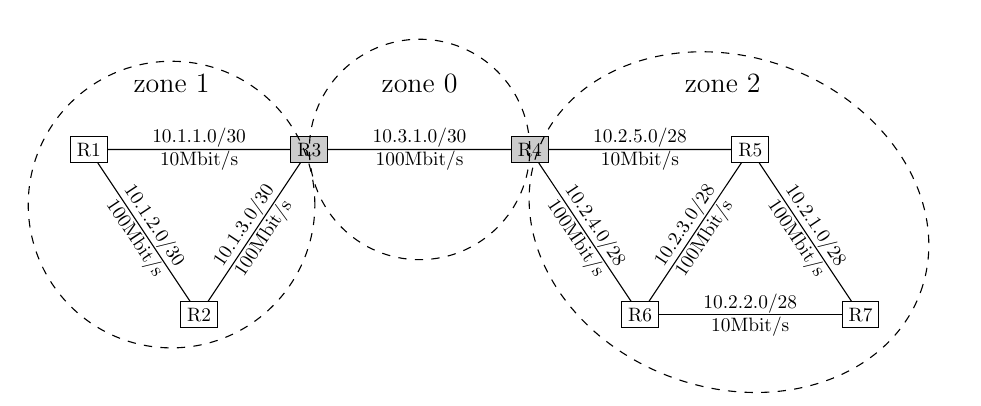
\begin{tikzpicture}[scale=0.7, transform shape]
        \node[draw] (R1) at (-6,3) {R1};
        \node[draw] (R2) at (-4,0) {R2};
        \node[draw, fill=gray!40] (R3) at (-2,3) {R3};
        \node[draw, fill=gray!40] (R4) at (2,3) {R4};
        \node[draw] (R5) at (6,3) {R5};
        \node[draw] (R6) at (4,0) {R6};
        \node[draw] (R7) at (8,0) {R7};
        \node (Z1) at (-4.5,4.2) {\Large{zone 1}};
        \node (Z0) at (0,4.2) {\Large{zone 0}};
        \node (Z2) at (5.5,4.2) {\Large{zone 2}};

        \draw (R1) -- (R3) node[midway,text width=1.8cm, text centered]{10.1.1.0/30 10Mbit/s};
        \draw (R1) -- (R2) node[sloped, midway,text width=1.8cm, text centered]{10.1.2.0/30 100Mbit/s};
        \draw (R3) -- (R2) node[sloped, midway,text width=1.8cm, text centered]{10.1.3.0/30 100Mbit/s};
        \draw (R3) -- (R4) node[midway,text width=1.8cm, text centered]{10.3.1.0/30 100Mbit/s};
        \draw (R4) -- (R5) node[midway,text width=1.8cm, text centered]{10.2.5.0/28 10Mbit/s};
        \draw (R4) -- (R6) node[sloped, midway,text width=1.8cm, text centered]{10.2.4.0/28 100Mbit/s};
        \draw (R5) -- (R6) node[sloped, midway,text width=1.8cm, text centered]{10.2.3.0/28 100Mbit/s};
        \draw (R7) -- (R6) node[midway,text width=1.8cm, text centered]{10.2.2.0/28 10Mbit/s};
        \draw (R5) -- (R7) node[sloped, midway,text width=1.8cm, text centered]{10.2.1.0/28 100Mbit/s};

        \draw[dashed] (0,3) circle (2) ;
        \draw[dashed] (-4.5,2) circle (2.6) ;
        \draw[dashed,rotate=-20] (4.7,3.5) ellipse (3.7 and 3) ;
    \end{tikzpicture}
\end{center}
\end{frame}
\begin{frame}
    \frametitle{Correction}
    Seconde étape: informations des autres zones
    \begin{center}
        \begin{tabular}{|*{4}{c|}}
            \hline
            Destination & Passerelle    & Interface & Coût \\
            \hline
            10.2.1.0/28 &               & 10.2.1.1  & 1    \\
            \hline
            10.2.2.0/28 & R7 & 10.2.1.1  & 11    \\
            \hline
            10.2.3.0/28 &               & 10.2.3.1  & 1   \\
            \hline
            10.2.4.0/28 & R6 & 10.2.3.1  & 2    \\
            \hline
            10.2.5.0/28 &  & 10.2.5.1  & 10    \\
            \hline
            10.3.1.0/30 & R6 & 10.2.3.1  & 3    \\
            \hline
            10.1.1.0/30 & R6 & 10.2.3.1  & 13    \\
            \hline
            10.1.3.0/30 & R6 & 10.2.3.1  & 4    \\
            \hline
            10.1.2.0/30 & R6 & 10.2.3.1  & 5    \\
            \hline
        \end{tabular}
        \captionof{table}{Table de routage de R5}
    \end{center}

\end{frame}
\section{Utilisation du protocole}
\begin{frame}
    \frametitle{Utilisation du protocole}

    \begin{itemize}
        \item<1-> OSPF est un protocole IGP (Interior Gateway Protocol), c'est-à-dire qu'il agit au sein d'un système autonome. Un fournisseur d'accès internet est un système autonome.
        \note[item]{un fournisseur peut donc \emph{en théorie} filtrer le contenu vers le client (c'est le cas pour les sites de dwl)}
        \item<2-> Pour assurer le routage entre les systèmes autonomes, un protocole de type EGP (Exterior Gateway Protocol) doit être mis en œuvre. Dans le cas de l'Internet, c'est généralement BGP (Border Gateway Protocol) qui assume cette mission.
        \note[item]{hors programme} 
    \end{itemize}

\end{frame}
\end{document}